
\documentclass[11pt,border=2mm]{standalone}

\usepackage{tikz}
\usepackage{nicefrac}
\usetikzlibrary{positioning}

\begin{document}
    
    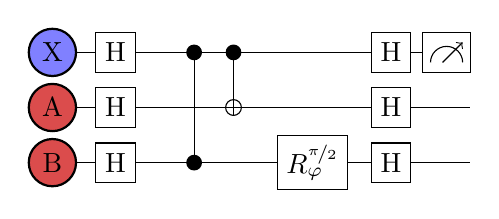
\begin{tikzpicture}[
    scale=1,
    pics/measure/.style 2 args={code={\draw[fill=white] (0,-#2/2) rectangle (#1,#2/2);\draw (1,-0.25) arc (0:180:0.4);\draw[->] (0.5,-0.25) -- (1,0.25);}},
    pics/dot/.style={code={\fill[black] (0,0) circle (0.1);}},
    pics/odot/.style={code={\fill[draw=black, fill=white] (0,0) circle (0.1); \draw (-0.1,0) -- (+0.1,0) (0,-0.1) -- (0,+0.1);}},
    pics/qubit/.style 2 args={code={\draw[black, thick, fill=#1] (-0.3,0) node[anchor=center] {#2} circle (0.3);}},
    ]
    %change these values:
    \pgfmathsetmacro{\linedist}{-0.7}
    \pgfmathsetmacro{\ep}{5}
    \pgfmathsetmacro{\ms}{0.5cm}



    \draw[] (0,0) pic[anchor=east] {qubit={blue!50}{X}}
    -- ++(0.5, 0) node[anchor=center, fill=white, draw=black, minimum size=\ms]{H}
    -- (4, 0) node[anchor=center, fill=white, draw=black, minimum size=\ms]{H}
    -- (\ep-0.6, 0) pic[anchor=center,scale=0.51] {measure={1.2}{1}};

    \draw[] (0,\linedist) pic[anchor=east] {qubit={red!80!black!70}{A}}
    -- ++(0.5, 0) node[anchor=center, fill=white, draw=black, minimum size=\ms]{H}
    -- (4, 1*\linedist) node[anchor=center, fill=white, draw=black, minimum size=\ms]{H}
    -- (\ep,\linedist) {};

    \draw[] (0,2*\linedist) pic[anchor=east] {qubit={red!80!black!70}{B}}
    -- ++(0.5, 0) node[anchor=center, fill=white, draw=black, minimum size=\ms]{H}
    -- ++(2.5, 0) node[anchor=center, fill=white, draw=black, minimum size=\ms]{$R_\mathrm{\varphi}^{\nicefrac{\pi}{2}}$}
    -- (4, 2*\linedist) node[anchor=center, fill=white, draw=black, minimum size=\ms]{H}
    -- (\ep,2*\linedist) {};

    \draw (1.5,0) pic[] {dot} -- ++ (0,2*\linedist){} pic[] {dot};
    \draw (2.0,0) pic[] {dot} -- ++ (0,1*\linedist){} pic[] {odot};
    \end{tikzpicture}
    % this is a test to test that this works
\end{document}